\documentclass[a4,10pt]{aleph-notas}

%% --> Paquetes adicionales
\usepackage{multicol}
\usepackage{marginnote}
\usepackage{metalogo}
%% --> Paquetes comunes
\usepackage{listings}
\usepackage{enumitem}
\usepackage{lipsum}
\usepackage{booktabs}
\usepackage{todonotes}
\usepackage[spanish,onelanguage,vlined,linesnumbered]{algorithm2e}
\setuptodonotes{color=colordef!40, size=\footnotesize}
\newcommand{\porhacer}[1]{\todo[inline]{\textbf{Por hacer:} #1}}

%% --> Definición de colores
\definecolor{codegreen}{HTML}{A5BE00}
\definecolor{codegray}{rgb}{0.5,0.5,0.5}
\definecolor{codepurple}{rgb}{0.58,0,0.82}
\definecolor{backcolour}{rgb}{0.95,0.95,0.92}

%% --> Estilo para código
\lstdefinestyle{mystyle}{
    language={[LaTeX]TeX}, % lenguaje
    basicstyle=\bfseries\ttfamily,
    keywordstyle=\color{colordef},
    commentstyle=\color{codegreen},
    inputencoding=utf8,
    showstringspaces=false,
    flexiblecolumns=true,
    stringstyle=\ttfamily\color{blue},
    extendedchars=true,
    emph={rm,bf,it,sf}, %...
    literate=%
    {ó}{{\'o}}1%
    {í}{{\'i}}1%
    {á}{{\'a}}1%
    {ú}{{\'u}}1%
}

%% --> Selección de estilo para el código
\lstset{
    style=mystyle,escapeinside={(*@}{@*)}
}

% Blancos tipográficos
\newcommand{\mq}{\hspace{0.5em}}  %medio cuadratín
\newcommand{\tq}{\hspace{0.33em}} % un terio de cuadratín
\newcommand{\qq}{\hspace{0.25em}} % un cuarto de cuadratín
\newcommand{\fs}{\hspace{0.125em}} % un octavo de cuadratín
\newcommand{\ep}{\hspace{0.05em}} % espacio de pelo

%% --> Nota para el material
\newcommand{\informacion}{\noindent{\small\color{colordef}
El presente material fue desarrollado por:

\begin{center}
\textbf{Daniel Lara}\\
\emph{Facultad de Ciencias, Escuela Politécnica Nacional}\\[2mm]


\textbf{Andrés Merino}\\
\emph{Facultad de Ciencias Exactas y Naturales, Pontificia Universidad Católica del Ecuador}
\end{center}

\medskip\noindent
La versión actual del material es 1.3-(Noviembre 2021). En caso de encontrar inconsistencias o errores en el presente material se pueden comunicar a \href{mailto:daniel.lara@alephsub0.org}{daniel.lara@alephsub0.org}. Para más información puedes visitar nuestro sitio web: \href{https://alephsub0.org}{alephsub0.org}. Si deseas colaborar con el desarrollo de este material, el código fuente está disponible en:   
\url{https://github.com/alephsub0/LaTeX_Guias.git}. Cualquier aporte (\emph{Pull request}) será de gran ayuda para mejorar este material. 

\medskip\noindent

\includegraphics[height=10pt]{Imagenes/CreativeCommos/cc.xlarge.png}

\includegraphics[height=10pt]{Imagenes/CreativeCommos/by.xlarge.png}

\includegraphics[height=10pt]{Imagenes/CreativeCommos/nc.xlarge.png}
Esta obra se encuentra bajo licencia Atribución-NoComercial-CompartirIgual 4.0 Internacional (CC BY-NC-SA 4.0) Para más información puede visitar: \url{https://creativecommons.org/licenses/by-nc-sa/4.0/}


%% -- > Aquí se incluyen los nombres de los colaboradores de estas guías:
% \medskip\noindent
% Otros colaboradores: Katheryn Yánes
}}

%%--> Formato para títulos
\titleformat{name=\section,numberless}[display]
  {\vspace*{-2mm}\bfseries\scshape\centering}
    {}{1ex}
    {\color{colortext}\large\titlerule\vspace{.05ex}
     }
    [\color{colortext}\vspace{.2ex}\titlerule]

\titleformat{\subsubsection}
    {\color{colortext}\normalsize\bfseries}
    {\thesubsubsection}{1em}{}
    
%% --> Datos de las guias
\universidad{Curso de \LaTeX}
\autor{Proyecto Alephsub0}
\materia{Introducción a \LaTeX}

%% --> Logos de las guias
\logouno[4.5cm]{Imagenes/Logos/LogoAlephsub0-02.png}
\longtitulo{0.6\linewidth}
\fecha{Noviembre de 2021}

%% --> Nuevos ambientes
% \definecolor{coloryt}{rgb}{0.769,0.188,0.169}
%% Ambientes
\makeatletter
%%  Keys temporales: |colorlat|
\def\tcb@@colorlat{colordef!50!black}
    \tcbset{ colorlat/.code = {\def\tcb@@colorlat{#1} } }
%%  Estilo de YouTube
\tcbset{ postitbeta/.style ={
    % -> Opciones generales
    breakable,enhanced,
    before skip=2mm,after skip=3mm,
    colback=\tcb@@color!50,colframe=\tcb@@color!20!black,
    boxrule=0.4pt,
    drop fuzzy shadow,
    left=6mm,right=2mm,top=0.5mm,bottom=0.5mm,
    sharp corners,rounded corners=southeast,arc is angular,arc=3mm,
    parbox=false,
    underlay unbroken and last = {%
        \path[fill=tcbcolback!80!black]
        ([yshift=3mm]interior.south east) --++ (-0.4,-0.1) --++ (0.1,-0.2);
        \path[draw=tcbcolframe,shorten <=-0.05mm,shorten >=-0.05mm]
        ([yshift=3mm]interior.south east) --++ (-0.4,-0.1) --++ (0.1,-0.2);
        \path[fill=\tcb@@colorlat,draw=none]
        (interior.south west) rectangle node[white]{\tcb@@icono} ([xshift=5.5mm]interior.north west);
        },
    underlay = {%
        \path[fill=\tcb@@colorlat,draw=none]
        (interior.south west) rectangle node[white]{\tcb@@icono} ([xshift=5.5mm]interior.north west);
        }
    }
    }
\makeatother

%% Recuadro para enlaces de YouTube
\definecolor{coloryt}{HTML}{ffcccc}
\newtcolorbox{tcbyoutube}
    {icono=\faYoutubePlay,color=coloryt,colorlat=red,postitbeta,colframe=red,leftright skip=1cm}
    
%% Comando para enlaces de YouTube
\newcommand{\YouTube}[4]%
    {
        \begin{tcbyoutube}
            \parbox{0.30\linewidth}{\href{#2}{\includegraphics[width=\linewidth]{#3}}}
            \hspace{2mm}
            \parbox{0.65\linewidth}{\footnotesize
            \textbf{#1}\\[1mm]
            \faLink\ \url{#2}\\[2mm]
            \scriptsize
            #4}
        \end{tcbyoutube}
    }
    
%% Recuadro para enlaces
\definecolor{coloren}{HTML}{B9F2BC}
\newtcolorbox{tcbenlace}
    {icono=\faLink,color=coloren,postit,leftright skip=1cm,fontupper=\small}

%% Recuadro para impresión
\definecolor{colorimp}{HTML}{F8F8FF}
\newtcolorbox{tcbimprimir}
    {icono=\faPrint,color=colorimp,postit,leftright skip=1cm,fontupper=\small}

%% Ambiente para código
\definecolor{colcod}{RGB}{174,218,255}
\newtcolorbox{tcbcodigo}
    {icono=\faCode,color=colcod,postit,top=-2mm,bottom=-2mm,leftright skip=1cm,fontupper=\small}

%% Ambiente para código LaTeX  
\usepackage{minted}
\usemintedstyle{borland}
\tcbuselibrary{minted}
\tcbset{listing engine=minted}
\newtcblisting{tcbLaTeX}{%
    icono=\faCode,color=colcod,postit,top=0mm,bottom=0mm,
    leftright skip=1cm,fontupper=\small,
    minted language=latex,minted style=colorful,
    listing only}
% \newtcolorbox{tcbcodigo}
%     {icono=\faCode,color=colcod,postit,top=-2mm,bottom=-2mm,leftright skip=1cm,fontupper=\small}

%% Ambiente para figuras 
\newtcolorbox[blend into=figures]{figura}[2][]
    {float=h,capture=hbox,title={#2},every float=\centering,
    arc=0mm,left=2mm,right=2mm,
    boxrule=0pt,
    colback=colordef!10,
    colbacktitle=colordef!80,fonttitle=\small,
    enhanced,attach boxed title to bottom,center title,
    #1}

%% Ambiente para tablas 
\newtcolorbox[blend into=tables]{tabla}[2][]
    {float=h,capture=hbox,title={#2},every float=\centering,
    arc=0mm,left=2mm,right=2mm,
    boxrule=0pt,
    colback=colordef!10,
    colbacktitle=colordef!80,fonttitle=\small,
    enhanced,center title,
    #1}

%% Ambiente para código LaTeX desplegado
\newtcblisting{tcbLaTeXb}{%
    icono=\faCode,color=colcod,postit,top=0mm,bottom=0mm,
    fontupper=\small,
    minted language=latex,minted style=colorful,listing side text}
\newtcblisting{tcbLaTeXs}{%
    icono=\faCode,color=colcod,postit,top=0mm,bottom=0mm,
    fontupper=\small,
    minted language=latex,minted style=colorful}

%% Recuadro para comando en línea
\DeclareTotalTCBox{\miverb}{ v }{
    fontupper=\ttfamily,nobeforeafter,tcbox raise base,arc=0pt,outer arc=0pt,
    top=0pt,bottom=0pt,left=0mm,right=0mm,
    leftrule=0pt,rightrule=0pt,toprule=0.3mm,bottomrule=0.3mm,boxsep=0.5mm,
    colback=colcod!10!white,colframe=colcod!50!black}{#1}


% -- Datos del libro
\nota{Guía 2}
\tema{Formato de texto, listas, cajas, fuentes}

%%--> Opciones adicionales

%%%%%%%%%%%%%%%%%%%%%%%%%%%%%%%%%%%%%%%%
%%%%%%%%%% Comienzo del documento
%%%%%%%%%%%%%%%%%%%%%%%%%%%%%%%%%%%%%%%%

\begin{document}

\encabezado

\informacion


\tableofcontents

\section{Introducción}

\LaTeX{} tiene una filosofía de trabajo diferente a la de los procesadores de texto habituales\footnote{Conocidos como \textsf{WYSIWYG}, es decir, «lo que ves es lo que obtienes»} y se basa en comandos. Tradicionalmente, este aspecto se ha considerado una desventaja (probablemente la única). Sin embargo, a diferencia de los procesadores de texto de tipo \textsf{WYSIWYG}, permite a quien escribe un documento centrarse exclusivamente en el contenido, sin tener que preocuparse de los detalles del formato. En este sentido, tampoco requiere de un programa específico para la edición del código pues esta tarea puede ser realizada en cualquier editor de texto plano requiriendo únicamente el compilador apropiado para obtener el resultado deseado.

\section{Escritura de texto}

\subsection{Títulos, capítulos y secciones}

\begin{advertencia}
En general, se debe permitir que \LaTeX{} de el formato a los títulos y subtítulos mediante los comandos de sección, sub-sección, etc.
\end{advertencia}

\LaTeX{} permite dividir el documento en capítulos, secciones y subsecciones mediante órdenes especiales que toman el título de la sección como argumento.

Las siguientes órdenes de división están disponibles para la clase \texttt{article}:
\begin{itemize}
\item \verb"\section{...}"
\item \verb"\subsection{...}"
\item \verb"\subsubsection{...}"
\item \verb"\paragraph{...}"
\item \verb"\subparagraph{...}"
\end{itemize}

Si se quiere dividir el documento en partes sin influir en la numeración de secciones o capítulos puede usar \verb|\part{...}|. Por otra parte, cuando se trabaje con las clases \texttt{report} o \texttt{book}, estará disponible una orden de sección adicional \verb|\chapter{...}|. En este caso, \LaTeX{} crea un índice general tomando los encabezados de sección y los números de página del último ciclo de compilación del documento.  La orden \verb"\tableofcontents" sitúa el índice general en el lugar en que se ejecuta la orden.  Un documento nuevo debe compilarse dos veces para conseguir un índice correcto\footnote{Esta aclaración es necesaria únicamente para procesos locales, es decir, cuando instalamos \LaTeX{} en nuestro computador. En el caso de \emph{Overleaf} el uso de ciertas herramientas internas hace que el documento se compile el número de veces que se requiera para obtener el documento completo.}
Todas las órdenes de sección listadas anteriormente tienen una versión «estrella».  Se trata de órdenes con el mismo nombre pero seguido de
un asterisco \verb|*|.  Generan encabezados de sección que no aparecen en el índice general y que no se numeran.


\begin{advertencia}
Una forma de revisar el contenido de la tabla de contenidos es verificar el archivo con extensión \texttt{.toc} este archivo contiene todas las entradas que serán utilizadas en el documento.
\end{advertencia}

Un ejemplo del contenido de este archivo lo podemos ver a continuación en el archivo \texttt{.toc} generado al compilar la presente guía.

\begin{figure}[H]
    \centering
    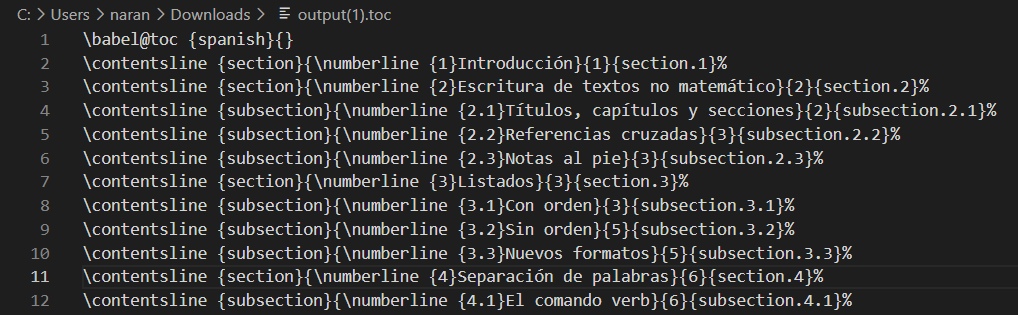
\includegraphics[width=0.90\textwidth]{Imagenes/guia02_1.png}
\end{figure}

Normalmente, los encabezados aparecen en el índice general exactamente como se introducen en el texto.  No obstante, a veces esto no es posible, porque el encabezado es demasiado largo y no cabe en el índice general.  Por tanto, la entrada para el índice general puede indicarse como un argumento opcional antes del encabezado real.

\begin{lstlisting}[frame=single]
\chapter[Título para el índice general]{Título real del capítulo}
\end{lstlisting}

El \emph{título} de todo el documento se genera con la orden \verb"\maketitle". El contenido del título tiene que definirse mediante las órdenes
 \begin{itemize}
  \item \verb|\title{...}|,
  \item \verb|\author{...}| y opcionalmente
  \item \verb|\date{...}|
 \end{itemize}
antes de llamar a \verb|\maketitle|.  En el argumento de \verb"\author", puede poner varios nombres separados por órdenes \verb"\and".

Además de las órdenes de sección ya explicadas, \LaTeXe{} tiene tres órdenes adicionales para usar con la clase \verb|book|, útiles
para dividir la publicación.  Las órdenes alteran los encabezados de los capítulos y los números de página para que aparezcan como se ve en
muchos libros:
 \begin{itemize}
  \item \verb|\frontmatter|: cambia la numeración de páginas a números romanos y las secciones no estarán numeradas.
  \item \verb|\mainmatter|: activa los números de página arábigos y reinicia el contador de páginas.
  \item \verb|\appendix|: tras esta orden los capítulos se numerarán con letras.
  \item \verb|\backmatter|: no tiene efecto visual en las clases típicas.
 \end{itemize}

  \subsection{Referencias cruzadas}

En libros, informes y artículos, hay a menudo \emph{referencias cruzadas} a figuras, cuadros y secciones especiales de texto, \LaTeX{} proporciona las siguientes órdenes para referenciar:
 \begin{itemize}
  \item \verb|\label{|\emph{marcador}\verb|}|,
  \item \verb|\ref{|\emph{marcador}\verb|}| ,
  \item \verb|\pageref{|\emph{marcador}\verb|}|
 \end{itemize}
donde \emph{marcador} es un identificador escogido por el usuario, \LaTeX{} remplaza \verb|\ref| por el número de la sección, subsección, figura, tabla o teorema tras el que se sitúa la orden \verb|\label| correspondiente. \verb|\pageref| imprime el número de página donde se encuentra el comando \verb|\label|.

  \subsection{Notas al pie}

Con la orden \verb|\footnote{|\emph{texto al pie}\verb|}| se imprime una nota al pie de la página actual.  Deben ponerse las notas tras la palabra u oración a la que se refieren. A continuación se encuentra un ejemplo sobre la generación de notas al pie:

\begin{lstlisting}[frame=single]
Aquí se va a generar una nota al pie.\footnote{Esta es la nota que hemos generado.}
\end{lstlisting}

\section{Listados}

Las listas son elementos básicos en un documento, para generarlas en \LaTeX \hspace{1.5pt} existen dos ambientes. El uso de uno u otro ambiente depende de si la lista posee un orden o no.

\subsection{Con orden}

Para las listas que poseen un orden se usa el ambiente \verb"enumerate", este ambiente genera una lista que enumera con un orden específico, el esquema de orden por defecto es:

\begin{itemize}
    \item
        Números arábigos (1, 2, 3, ...) para el nivel 1,
    \item
        letras minúsculas (a, b, c, ...) para el nivel 2,
    \item
        números romanos en minúscula (i, ii, iii, ...) para el nivel 3,
    \item
        letras mayúsculas (A, B, C, ...) para el nivel 4. 
\end{itemize}

Así, consideremos el siguiente ejemplo:

\begin{lstlisting}[frame=single]
 \begin{enumerate}
   \item 
        Item de primer nivel
   \item
        Item de primer nivel
   \begin{enumerate}
    \item
        Segundo nivel item
    \item
        Segundo nivel item
     \begin{enumerate}
       \item Item de tercer nivel
       \item Item de tercer nivel
       \begin{enumerate}
         \item Item de cuarto nivel
         \item Item de cuarto nivel
       \end{enumerate}
     \end{enumerate}
   \end{enumerate}
 \end{enumerate}
\end{lstlisting}

produce:

\begin{center}
{ \fboxsep 12pt
\fcolorbox {black}{white}{
\begin{minipage}[t]{10cm}
\begin{enumerate}
   \item Item de primer nivel
   \item Item de primer nivel
   \begin{enumerate}
     \item Item de segundo nivel
     \item Item de segundo nivel
     \begin{enumerate}[label=\roman*.]
       \item Item de tercer nivel
       \item Item de tercer nivel
       \begin{enumerate}[label=\Alph*.]
         \item Item de cuarto nivel
         \item Item de cuarto nivel
       \end{enumerate}
     \end{enumerate}
   \end{enumerate}
 \end{enumerate}
\end{minipage}
} }
\end{center}

De igual manera, se tienen los siguientes ejemplos:

\begin{lstlisting}[frame=single]
\begin{enumerate}
    \item
        Primero
    \item
        Segundo
    \item
        Tercero
        \begin{enumerate}
        \item
            Tercero, uno.
        \item
            Tercero, dos.
        \end{enumerate}
\end{enumerate}
\end{lstlisting}

produce:

\begin{center}
{ \fboxsep 12pt
\fcolorbox {black}{white}{
\begin{minipage}[t]{10cm}
\begin{enumerate}
    \item
        Primero
    \item
        Segundo
    \item
        Tercero
        \begin{enumerate}
        \item
            Tercero, uno.
        \item
            Tercero, dos.
        \end{enumerate}
\end{enumerate}
\end{minipage}
} }
\end{center}

%%%%%%%%%%%%%%%%%%%%%%%
\subsection{Sin orden}

Para las listas que no tienen orden se usa el ambiente \verb"itemize", este ambiente genera una lista que enumera sin orden específico. Un ejemplo es:

\begin{lstlisting}[frame=single]
\begin{itemize}
    \item 
        Una cosa
    \item 
        Otra cosa
\end{itemize}
\end{lstlisting}

produce:

\begin{center}
{ \fboxsep 12pt
\fcolorbox {black}{white}{
\begin{minipage}[t]{10cm}
\begin{itemize}
    \item 
        Una cosa
    \item 
        Otra cosa
\end{itemize}
\end{minipage}
} }
\end{center}

\subsection{Nuevos formatos}

\subsubsection{Formatos temporales}

Adicionalmente, es posible crear numeraciones personalizadas usando los siguientes estilos disponibles:

\begin{center}
    \begin{tabular}{c|c}
        Código & Descripción \\
        \hline
        \verb"\alph" & Letras en minúscula (a,b,$\ldots$)\\ 
        \verb"\Alph" & Letras en Mayúscula (A,B,$\ldots$)\\
        \verb"\arabic" & Números arábigos ($1,2,\ldots$)\\
        \verb"\roman" & Números romanos en minúscula (i,ii,$\ldots$)\\
        \verb"\Roman"   & Números romanos en Mayúscula (I,II,$\ldots$)
    \end{tabular}
\end{center}

para definir el formato de numeración veamos el siguiente ejemplo:

\begin{lstlisting}[frame=single]
\begin{enumerate}[label=\textbf{1.\arabic*)}]
    \item 
        Primero
    \item 
        Segundo
    \item 
        Tercero
            \begin{enumerate}[label=\roman*.]
                \item 
                    Tercero, uno.
                \item 
                    Tercero, dos.
            \end{enumerate}
\end{enumerate}
\end{lstlisting}

produce:

\begin{center}
{ \fboxsep 12pt
\fcolorbox {black}{white}{
\begin{minipage}[t]{10cm}
\begin{enumerate}[label=\textbf{1.\arabic*)}]
    \item 
        Primero
    \item 
        Segundo
    \item 
        Tercero
            \begin{enumerate}[label=\roman*.]
                \item 
                    Tercero, uno.
                \item 
                    Tercero, dos.
            \end{enumerate}
\end{enumerate}
\end{minipage}
} }
\end{center}

\subsubsection{Formatos globales}

En la subsección anterior vimos como modificar las etiquetas de una lista de manera local, es decir, el cambio solo afecta a la lista en cuestión, mientras el resto del documento permanece sin cambios; en el caso de que se desee realizar un cambio global, debemos modificar las variables de etiqueta; un ejemplo de esto se encuentra a continuación:

\begin{lstlisting}[frame=single]
\renewcommand{\labelenumi}{\arabic{enumi}.}
\renewcommand{\labelenumii}{\arabic{enumi}.\arabic{enumii}}
\renewcommand{\labelenumiii}{\arabic{enumi}.\arabic{enumii}.\arabic{enumiii}}

\begin{enumerate}
    \item
        Primero
    \item
        Segundo
    \item
        Tercero
        \begin{enumerate}
        \item
            Tercero, uno.
        \item
            Tercero, dos.
            \begin{enumerate}
                \item Tercero, dos uno.
            \end{enumerate}
        \end{enumerate}
\end{enumerate}
\end{lstlisting}

\noindent
Esto produce:

\begin{center}
{ \fboxsep 12pt
\fcolorbox {black}{white}{
\begin{minipage}[t]{10cm}
\begin{enumerate}[label=\arabic*.]
    \item
        Primero
    \item
        Segundo
    \item
        Tercero
        \begin{enumerate}[label=\arabic{enumi}.\arabic{enumii}]
        \item
            Tercero, uno.
        \item
            Tercero, dos.
            \begin{enumerate}[label=\arabic{enumi}.\arabic{enumii}.\arabic{enumiii}]
                \item Tercero, dos uno.
            \end{enumerate}
        \end{enumerate}
\end{enumerate}
\end{minipage}
} }
\end{center}

\subsection{Texto subrayado}

Para obtener el texto subrayado seguimos la siguiente sintaxis

\begin{lstlisting}[frame=single]
\underline{Subrayado}
\end{lstlisting}

\begin{center}
{ \fboxsep 12pt
\fcolorbox {black}{white}{
\begin{minipage}[t]{1.8cm}
\underline{Subrayado}
\end{minipage}
} }
\end{center}


\section{Cajas}

Para encerrar el texto o un objeto en una caja podemos usar los comandos \verb@\fbox{@\emph{objeto}\verb@}@ o \verb@\framebox{@\emph{objeto}\verb@}@. Un ejemplo lo podemos encontrar a continuación:

\begin{lstlisting}[frame=single]
Este documento está hecho en:\\
\fbox{\LaTeX}
\end{lstlisting}

\begin{center}
Este documento está hecho en:\\
\fbox{\LaTeX}
\end{center}

\section{Texto en varias columnas}

En muchas ocasiones es necesario escribir texto en varias columnas, por lo que existen diversas maneras para realizar esto. Así, vamos a analizar algunas de las opciones disponibles en \LaTeX{} para este fin.

\subsection{Multicol}

El paquete \verb@\multicol@ es uno de ellos, su sintaxis es bastante sencilla y se basa únicamente en incluir el paquete en el preámbulo y todo el texto que deseemos en columnas se escribe entre  \verb@\begin{multicol}{#}@ y \verb@\end{multicol}@. Notemos que el número de columnas estará dado por el parámetro <<\#>> en la segunda llave del ambiente.

\begin{lstlisting}[frame=single]
\begin{multicols}{3}
    \lipsum[1]
\end{multicols}
\end{lstlisting}

\begin{center}
{ \fboxsep 12pt
\fcolorbox {black}{white}{
\begin{minipage}[t]{15cm}
    \begin{multicols}{3}
    \lipsum[1]
    \end{multicols}
\end{minipage}
} }
\end{center}

\subsection{Minipage}

El ambiente minipage permite crear <<mini secciones>> que guardan cierta independencia del documento en general, permitiendo ajustar algunos parámetros a manera de un recuadro.

\begin{lstlisting}[frame=single]
\begin{minipage}[b]{0.45\textwidth}
    \lipsum[1]
\end{minipage} \hfill \begin{minipage}[b]{0.45\textwidth}
    \lipsum[1]
\end{minipage}
\end{lstlisting}

\bigskip
\bigskip

\begin{minipage}[b]{0.45\textwidth}
Lorem ipsum dolor sit amet, consectetur adipiscing elit. Ut enim neque, pretium sit amet risus sit amet, vulputate hendrerit risus. Nam quis mi ullamcorper, dapibus nulla nec, hendrerit dolor. Aliquam varius velit a elementum porta. Nam sollicitudin erat sed nibh tincidunt venenatis. Sed scelerisque, est vitae maximus feugiat, massa metus facilisis sapien, cursus rutrum dolor ex ut felis. Aenean vestibulum dui vel urna varius, in bibendum sem iaculis. Aliquam a tempus lorem, vel efficitur felis. 
\end{minipage} \hfill \begin{minipage}[b]{0.45\textwidth}
Lorem ipsum dolor sit amet, consectetur adipiscing elit. Ut enim neque, pretium sit amet risus sit amet, vulputate hendrerit risus. Nam quis mi ullamcorper, dapibus nulla nec, hendrerit dolor. Aliquam varius velit a elementum porta. Nam sollicitudin erat sed nibh tincidunt venenatis. Sed scelerisque, est vitae maximus feugiat, massa metus facilisis sapien, cursus rutrum dolor ex ut felis. Aenean vestibulum dui vel urna varius, in bibendum sem iaculis. Aliquam a tempus lorem, vel efficitur felis. 
\end{minipage}

\section{Texto como en pantalla}

\subsection{Comando \emph{verb}}

En ocasiones, resulta necesario mostrar el código tal y como lo vemos en el editor, como es el caso de este documento, una primera opción para realizar esto es utilizar el comando \verb@\verb@ este nos muestra el texto tal y como lo vemos en el editor.

\begin{lstlisting}[frame=single]
\verb@\textbf{\textit{Este es un texto en negrita}}@
\end{lstlisting}

El código anterior produce:

\begin{center}
{ \fboxsep 12pt
\fcolorbox {black}{white}{
\begin{minipage}[t]{4.4cm}
\textbf{\textit{Este es un texto en negrita}}
\end{minipage}
} }
\end{center}

\subsection{Ambiente \emph{verbatim}}

Existen casos en los que deseamos mostrar el texto tal y como nosotros lo observamos en la pantalla de nuestro computador, notemos que por la estructura de \LaTeX{} es necesario el uso del ambiente \verb@verbatim@.

\begin{lstlisting}[frame=single]
\begin{verbatim}
    #include<iostream>
    #include<cmath>
    #include<sstream>
    using namespace std;
    int main()
    {       
        int x1,x2,x3,x4;
        int max;
        cout << "Ingrese 4 numeros \n";
        cin >> x1>>x2>>x3>>x4;
        max = x1;
        if (x2 > max){
            max =x2;
        }
        if (x3 > max){
            max =x3;
        }
        if (x4 > max){
            max =x4;
        }
        cout << "El maximo es: "<< max<<"\n";
        return 0;
    }
\end{verbatim}
\end{lstlisting}

\noindent
\begin{verbatim}
    #include<iostream>
    #include<cmath>
    #include<sstream>
    using namespace std;
    int main()
    {       
        int x1,x2,x3,x4;
        int max;
        cout << "Ingrese 4 numeros \n";
        cin >> x1>>x2>>x3>>x4;
        max = x1;
        if (x2 > max){
            max =x2;
        }
        if (x3 > max){
            max =x3;
        }
        if (x4 > max){
            max =x4;
        }
        cout << "El maximo es: "<< max<<"\n";
        return 0;
    }
\end{verbatim}


\subsection{Paquete \emph{listings}}

Este paquete provee opciones más avanzadas respecto a la inclusión de código; sin embargo, no profundizaremos más sobre este paquete en la presente guía. Para más información sobre este paquete puede consultar: \href{https://es.overleaf.com/learn/latex/Code_listing}{https://es.overleaf.com/learn/latex/Code\_listing} o en la documentación del paquete existente en CTAN.

\section{Lineas y efectos de texto}

En esta sección encontraremos algunas herramientas útiles para el formateo de textos. Por ejemplo:

\subsection{\texttt{hfill}}

\begin{lstlisting}[frame=single]
\textsc{Escuela Politecnica Nacional} \hfill Semestre 2019-B
\end{lstlisting}

\begin{center}
{ \fboxsep 12pt
\fcolorbox {black}{white}{
\begin{minipage}[t]{0.9\textwidth}
    \textsc{Escuela Politécnica Nacional} \hfill Semestre 2019-B
\end{minipage}
} }
\end{center}

\subsection{\texttt{hrulefill} y \texttt{dotfill}}

\begin{lstlisting}[frame=single]
 Nombre: \hrulefill
\end{lstlisting}

\begin{center}
{ \fboxsep 12pt
\fcolorbox {black}{white}{
\begin{minipage}[t]{0.9\textwidth}  
    Nombre: \hrulefill
\end{minipage}
} }
\end{center}

\vspace{12pt}

\begin{lstlisting}[frame=single]
 \textsc{Escuela Politecnica Nacional \hfill Semestre 2019-B}\\
\rule[0.5cm]{\textwidth}{0.01cm}
\end{lstlisting}

\begin{center}
{ \fboxsep 12pt
\fcolorbox {black}{white}{
\begin{minipage}[t]{0.9\textwidth}
    \textsc{Escuela Politécnica Nacional \hfill Semestre 2019-B}\\
\rule[0.5cm]{\textwidth}{0.01cm}
\end{minipage}
} }
\end{center}



\section{Notas al margen}

Para realizar anotaciones al margen podemos emplear desde un uso adecuado del comando \verb@\hspace{}@ hasta paquetes especializados en crear este tipo de anotaciones. Así, veamos algunos métodos:

\subsection{Comando \emph{marginpar}}

Este comando nos permite agregar notas al margen aunque la presentación de las mismas dependen de las opciones especificadas en el paquete \verb@geometry@. A continuación se encuentra un breve ejemplo.

\bigskip

\marginnote{Esta es una anotación al margen}

\begin{lstlisting}[frame=single]
    \marginnote{Esta es una anotacion al margen}
\end{lstlisting}

\subsection{Comando \emph{hspace}}

Una forma de incluir notas al margen de manera «manual» consiste en abusar del comando \verb@\hspace@ y mover el texto deseado fuera del espacio de trabajo del documento. Un ejemplo se encuentra a continuación:

\begin{lstlisting}[frame=single]
    \hspace*{-2.2cm} {\cyan \small Texto} $\longrightarrow$
\end{lstlisting}

\hspace*{-2.2cm} {\color{cyan} \small Texto $\longrightarrow$}

\subsection{Paquete \emph{Marginnote}}

Para un mejor control sobre las notas al margen se puede usar este paquete que permite modificar la posición de las notas y algunos atributos adicionales. Más información sobre el funcionamiento de este paquete se puede encontrar en su documentación: \href{https://ctan.org/pkg/marginnote}{https://ctan.org/pkg/marginnote}.

\begin{lstlisting}[frame=single]
    Existen muchas notaciones para la derivada de una función. 
    \marginnote{$\frac{d}{dx}$\\$f'(x)$}
\end{lstlisting}

Existen muchas notaciones para la derivada de una función. \marginnote{$\frac{d}{dx}$\\$f'(x)$}

\section{Listas \textit{(Continuación)}}

En ocasiones suele ser necesario continuar la numeración de las listas, para realizar esto vamos a usar la opción \texttt{resume}

\begin{lstlisting}[frame=single]
    \begin{enumerate}[series = ejercicios]
        \item 
            Uno
        \item
            Dos
        \item
            Tres
    \end{enumerate}
    
    \begin{enumerate}[resume* = ejercicios]
        \item 
            Cuatro
        \item
            Cinco
    \end{enumerate}
\end{lstlisting}

\begin{enumerate}[series = ejercicios]
    \item 
        Uno
    \item
        Dos
    \item
        Tres
\end{enumerate}

\begin{enumerate}[resume* = ejercicios]
    \item 
        Cuatro
    \item
        Cinco
\end{enumerate}

\end{document} 